\newcommand{\RevisionTaxonomy}{%
\begin{table*}[t]\centering
\caption{Attack labels and potential service consequences in the derived subset.}\label{tab:attacks}
\resizebox{\textwidth}{!}{\begin{tabular}{lrrrr}\hline
Label & Client & Records & Possible service impact & Source\\\hline
BT-DoS & bluetooth & 6,735 & Gaps in wearable observations & \cite{dadkhah2024towards}\\
MQTT-DDoS-Connect\_Flood & mqtt & 17,264 & Less broker capacity for legitimate sessions & \cite{dadkhah2024towards}\\
MQTT-DDoS-Publish\_Flood & mqtt & 4,179 & Delayed monitoring topic updates & \cite{dadkhah2024towards}\\
MQTT-DoS-Connect\_Flood & mqtt & 2,707 & Less broker capacity for legitimate sessions & \cite{dadkhah2024towards}\\
MQTT-DoS-Publish\_Flood & mqtt & 5,411 & Delayed monitoring topic updates & \cite{dadkhah2024towards}\\
MQTT-Malformed\_Data & mqtt & 2,047 & Application endpoint processing errors & \cite{dadkhah2024towards}\\
ARP\_Spoofing & wifi & 1,584 & Misdirection of gateway-bound telemetry & \cite{dadkhah2024towards}\\
Recon-OS\_Scan & wifi & 1,611 & Discovery of exposed monitoring services & \cite{dadkhah2024towards}\\
Recon-Ping\_Sweep & wifi & 926 & Discovery of exposed monitoring services & \cite{dadkhah2024towards}\\
Recon-Port\_Scan & wifi & 2,432 & Discovery of exposed monitoring services & \cite{dadkhah2024towards}\\
Recon-VulScan & wifi & 1,444 & Discovery of exposed monitoring services & \cite{dadkhah2024towards}\\
TCP\_IP-DDoS-ICMP & wifi & 19,440 & Contention with monitor traffic & \cite{dadkhah2024towards}\\
TCP\_IP-DDoS-SYN & wifi & 10,721 & Contention with monitor traffic & \cite{dadkhah2024towards}\\
TCP\_IP-DDoS-TCP & wifi & 10,842 & Contention with monitor traffic & \cite{dadkhah2024towards}\\
TCP\_IP-DDoS-UDP & wifi & 20,498 & Contention with monitor traffic & \cite{dadkhah2024towards}\\
TCP\_IP-DoS-ICMP & wifi & 6,330 & Contention with monitor traffic & \cite{dadkhah2024towards}\\
TCP\_IP-DoS-SYN & wifi & 6,577 & Contention with monitor traffic & \cite{dadkhah2024towards}\\
TCP\_IP-DoS-TCP & wifi & 5,831 & Contention with monitor traffic & \cite{dadkhah2024towards}\\
TCP\_IP-DoS-UDP & wifi & 8,143 & Contention with monitor traffic & \cite{dadkhah2024towards}\\
\hline\end{tabular}}
\end{table*}
}

\newcommand{\RevisionTopology}{%
\begin{figure*}[t]\centering
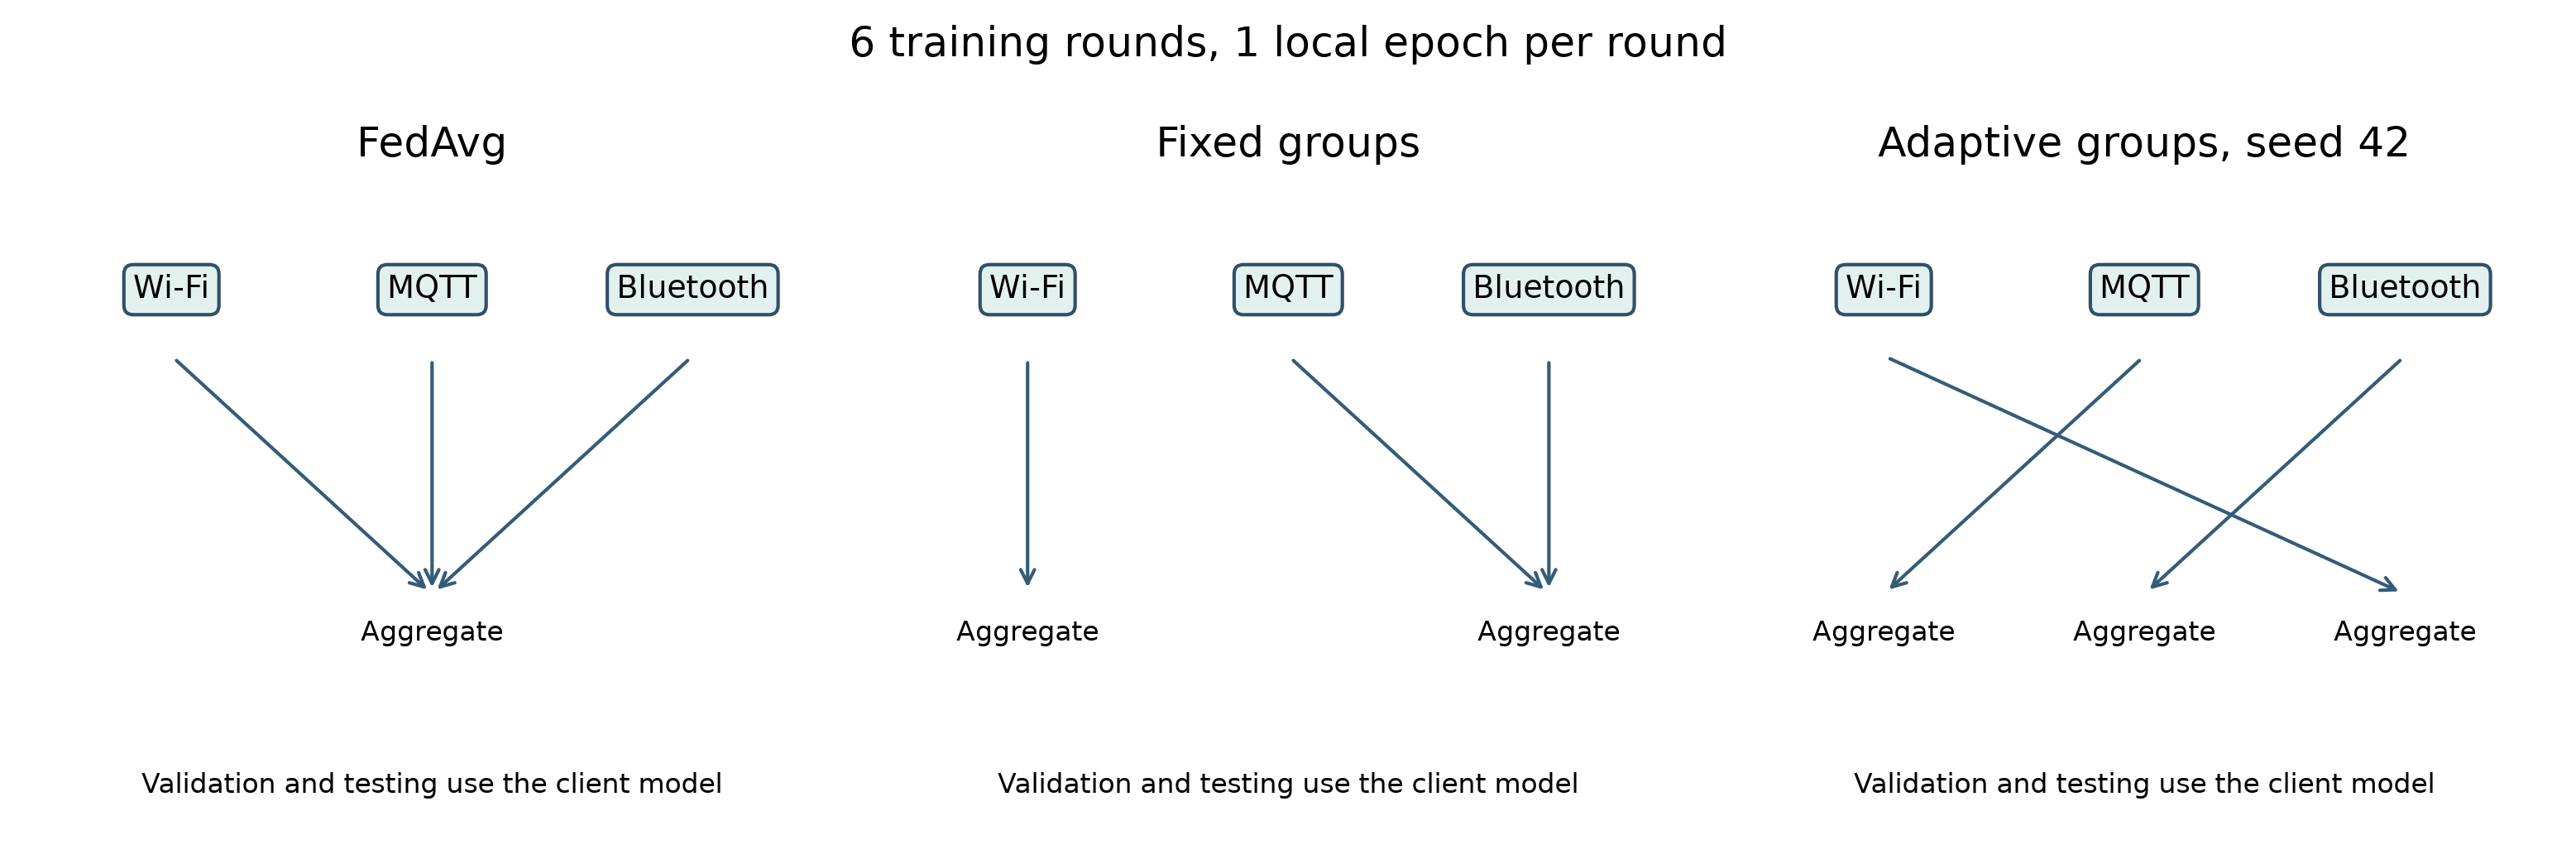
\includegraphics[width=0.93\textwidth]{revision_topology.png}
\caption{Training and parameter exchange by aggregation policy. Raw features stay with each simulated client during federated training. FedPer additionally retains its classification head locally. Pooled training is an offline comparator.}\label{fig:revised_topology}
\end{figure*}

\begin{table}[t]\centering
\caption{Adaptive group membership at each validation-selected checkpoint.}\label{tab:newgroups}
\small\begin{tabular}{lr}\hline
Seed & Client grouping\\\hline
42 & mqtt / bluetooth / wifi\\
7 & mqtt / bluetooth / wifi\\
123 & mqtt / bluetooth / wifi\\
2024 & mqtt / bluetooth / wifi\\
31337 & mqtt / bluetooth / wifi\\
\hline\end{tabular}
\end{table}
}

\newcommand{\RevisionDetection}{%
\begin{table*}[t]\centering
\caption{Grouped evaluation across 5 matched seeds. Entries are means and sample standard deviations.}\label{tab:newmain}
\resizebox{\textwidth}{!}{\begin{tabular}{lrrrr}\hline
Method & Client mean macro F1 & Pooled macro F1 & Bluetooth benign recall & Optimizer steps\\\hline
Adaptive groups & 0.9634 $\pm$ 0.0020 & 0.9768 $\pm$ 0.0014 & 0.9944 $\pm$ 0.0017 & 2349.6000 $\pm$ 3.2863\\
Centralized & 0.9639 $\pm$ 0.0022 & 0.9772 $\pm$ 0.0014 & 0.9963 $\pm$ 0.0014 & 2347.2000 $\pm$ 2.6833\\
Compute-matched centralized & 0.9641 $\pm$ 0.0024 & 0.9772 $\pm$ 0.0015 & 0.9964 $\pm$ 0.0013 & 2349.6000 $\pm$ 3.2863\\
Class-balanced loss & 0.7116 $\pm$ 0.0671 & 0.7878 $\pm$ 0.0395 & 0.2478 $\pm$ 0.2542 & 2349.6000 $\pm$ 3.2863\\
Equal client weights & 0.9097 $\pm$ 0.0021 & 0.9266 $\pm$ 0.0038 & 0.9592 $\pm$ 0.0084 & 2349.6000 $\pm$ 3.2863\\
FedAvg & 0.6376 $\pm$ 0.0458 & 0.7022 $\pm$ 0.0677 & 0.0161 $\pm$ 0.0214 & 2349.6000 $\pm$ 3.2863\\
FedPer & 0.8726 $\pm$ 0.0242 & 0.8949 $\pm$ 0.0196 & 0.7180 $\pm$ 0.1016 & 2349.6000 $\pm$ 3.2863\\
FedProx 0.001 & 0.6818 $\pm$ 0.0179 & 0.7667 $\pm$ 0.0105 & 0.0350 $\pm$ 0.0387 & 2349.6000 $\pm$ 3.2863\\
FedProx 0.01 & 0.6836 $\pm$ 0.0085 & 0.7820 $\pm$ 0.0050 & 0.0214 $\pm$ 0.0191 & 2349.6000 $\pm$ 3.2863\\
FedProx 0.05 & 0.6751 $\pm$ 0.0062 & 0.7779 $\pm$ 0.0068 & 0.0157 $\pm$ 0.0111 & 2349.6000 $\pm$ 3.2863\\
FedProx 0.1 & 0.6697 $\pm$ 0.0060 & 0.7725 $\pm$ 0.0080 & 0.0137 $\pm$ 0.0105 & 2349.6000 $\pm$ 3.2863\\
FedProx 0 & 0.6376 $\pm$ 0.0458 & 0.7022 $\pm$ 0.0677 & 0.0161 $\pm$ 0.0214 & 2349.6000 $\pm$ 3.2863\\
Fixed groups & 0.9604 $\pm$ 0.0026 & 0.9755 $\pm$ 0.0014 & 0.9827 $\pm$ 0.0028 & 2349.6000 $\pm$ 3.2863\\
Local-only & 0.9626 $\pm$ 0.0017 & 0.9768 $\pm$ 0.0012 & 0.9965 $\pm$ 0.0014 & 2349.6000 $\pm$ 3.2863\\
\hline\end{tabular}}
\end{table*}

\begin{table*}[t]\centering
\caption{Grouped test results for seed 42. BT denotes Bluetooth.}\label{tab:newseed42}
\resizebox{\textwidth}{!}{\begin{tabular}{lrrrrrrr}\hline
Method & Wi-Fi F1 & MQTT F1 & BT F1 & Wi-Fi benign & MQTT benign & BT benign & Client mean\\\hline
Adaptive groups & 0.9363 & 0.9694 & 0.9841 & 0.8368 & 0.9700 & 0.9947 & 0.9633\\
Centralized & 0.9359 & 0.9697 & 0.9867 & 0.8148 & 0.9628 & 0.9973 & 0.9641\\
Compute-matched centralized & 0.9359 & 0.9697 & 0.9867 & 0.8148 & 0.9628 & 0.9973 & 0.9641\\
Class-balanced loss & 0.8351 & 0.8218 & 0.4043 & 0.9986 & 0.6336 & 0.1151 & 0.6871\\
Equal client weights & 0.8549 & 0.9077 & 0.9643 & 0.9835 & 0.8101 & 0.9570 & 0.9090\\
FedAvg & 0.9201 & 0.7533 & 0.3022 & 0.9438 & 0.4710 & 0.0106 & 0.6586\\
FedPer & 0.9324 & 0.8375 & 0.7223 & 0.8848 & 0.6440 & 0.5459 & 0.8307\\
FedProx 0.001 & 0.9140 & 0.7913 & 0.2942 & 0.9492 & 0.5400 & 0.0032 & 0.6665\\
FedProx 0.01 & 0.9065 & 0.8268 & 0.2942 & 0.9630 & 0.6093 & 0.0032 & 0.6758\\
FedProx 0.05 & 0.8897 & 0.8144 & 0.2981 & 0.9767 & 0.5905 & 0.0069 & 0.6674\\
FedProx 0.1 & 0.8872 & 0.8020 & 0.2968 & 0.9753 & 0.5721 & 0.0058 & 0.6620\\
FedProx 0 & 0.9201 & 0.7533 & 0.3022 & 0.9438 & 0.4710 & 0.0106 & 0.6586\\
Fixed groups & 0.9362 & 0.9705 & 0.9750 & 0.8505 & 0.9856 & 0.9830 & 0.9606\\
Local-only & 0.9345 & 0.9705 & 0.9831 & 0.8395 & 0.9735 & 0.9979 & 0.9627\\
\hline\end{tabular}}
\end{table*}

\begin{table*}[t]\centering
\caption{Grouped test results for seed 7. BT denotes Bluetooth.}\label{tab:newseed7}
\resizebox{\textwidth}{!}{\begin{tabular}{lrrrrrrr}\hline
Method & Wi-Fi F1 & MQTT F1 & BT F1 & Wi-Fi benign & MQTT benign & BT benign & Client mean\\\hline
Adaptive groups & 0.9352 & 0.9760 & 0.9846 & 0.8230 & 0.9850 & 0.9949 & 0.9652\\
Centralized & 0.9365 & 0.9763 & 0.9842 & 0.8385 & 0.9780 & 0.9974 & 0.9657\\
Compute-matched centralized & 0.9382 & 0.9764 & 0.9855 & 0.8385 & 0.9790 & 0.9974 & 0.9667\\
Class-balanced loss & 0.8451 & 0.8122 & 0.5926 & 0.9986 & 0.6092 & 0.3524 & 0.7500\\
Equal client weights & 0.8489 & 0.9170 & 0.9701 & 0.9705 & 0.8353 & 0.9645 & 0.9120\\
FedAvg & 0.8975 & 0.7338 & 0.2870 & 0.9143 & 0.4397 & 0.0005 & 0.6395\\
FedPer & 0.9291 & 0.8643 & 0.8782 & 0.8596 & 0.7092 & 0.8138 & 0.8905\\
FedProx 0.001 & 0.9045 & 0.7954 & 0.2886 & 0.9129 & 0.5499 & 0.0021 & 0.6629\\
FedProx 0.01 & 0.8940 & 0.8383 & 0.2880 & 0.9129 & 0.6334 & 0.0015 & 0.6734\\
FedProx 0.05 & 0.8717 & 0.8502 & 0.2876 & 0.9256 & 0.6584 & 0.0010 & 0.6698\\
FedProx 0.1 & 0.8672 & 0.8441 & 0.2882 & 0.9368 & 0.6490 & 0.0015 & 0.6665\\
FedProx 0 & 0.8975 & 0.7338 & 0.2870 & 0.9143 & 0.4397 & 0.0005 & 0.6395\\
Fixed groups & 0.9357 & 0.9743 & 0.9798 & 0.8216 & 0.9962 & 0.9866 & 0.9633\\
Local-only & 0.9366 & 0.9762 & 0.9820 & 0.8301 & 0.9890 & 0.9974 & 0.9649\\
\hline\end{tabular}}
\end{table*}

\begin{table*}[t]\centering
\caption{Source-label supports and binary detector recall, seed 42.}\label{tab:newsupport}
\resizebox{\textwidth}{!}{\begin{tabular}{lrrrrrr}\hline
Label & Client & Train & Validation & Test & FedAvg recall & FedPer recall\\\hline
BT-DoS & bluetooth & 4075 & 1352 & 1308 & 0.9992 & 0.9809\\
Benign & bluetooth & 5800 & 1926 & 1885 & 0.0106 & 0.5459\\
Benign & mqtt & 10970 & 3680 & 3739 & 0.4710 & 0.6440\\
MQTT-DDoS-Connect\_Flood & mqtt & 10410 & 3357 & 3497 & 1.0000 & 1.0000\\
MQTT-DDoS-Publish\_Flood & mqtt & 2440 & 849 & 890 & 1.0000 & 1.0000\\
MQTT-DoS-Connect\_Flood & mqtt & 1593 & 568 & 546 & 1.0000 & 1.0000\\
MQTT-DoS-Publish\_Flood & mqtt & 3212 & 1105 & 1094 & 1.0000 & 1.0000\\
MQTT-Malformed\_Data & mqtt & 1202 & 422 & 423 & 0.9905 & 0.8251\\
ARP\_Spoofing & wifi & 956 & 312 & 316 & 0.7247 & 0.8259\\
Benign & wifi & 2169 & 716 & 729 & 0.9438 & 0.8848\\
Recon-OS\_Scan & wifi & 1006 & 294 & 311 & 0.9035 & 0.9293\\
Recon-Ping\_Sweep & wifi & 533 & 214 & 179 & 0.7877 & 0.9665\\
Recon-Port\_Scan & wifi & 1417 & 529 & 486 & 0.9691 & 0.9794\\
Recon-VulScan & wifi & 900 & 278 & 266 & 0.8722 & 0.9398\\
TCP\_IP-DDoS-ICMP & wifi & 11963 & 3606 & 3871 & 1.0000 & 1.0000\\
TCP\_IP-DDoS-SYN & wifi & 6449 & 2147 & 2125 & 0.9995 & 1.0000\\
TCP\_IP-DDoS-TCP & wifi & 6445 & 2278 & 2119 & 1.0000 & 1.0000\\
TCP\_IP-DDoS-UDP & wifi & 12345 & 4059 & 4094 & 0.9998 & 1.0000\\
TCP\_IP-DoS-ICMP & wifi & 3866 & 1215 & 1249 & 1.0000 & 1.0000\\
TCP\_IP-DoS-SYN & wifi & 3953 & 1324 & 1300 & 0.9992 & 1.0000\\
TCP\_IP-DoS-TCP & wifi & 3526 & 1142 & 1163 & 1.0000 & 1.0000\\
TCP\_IP-DoS-UDP & wifi & 4876 & 1619 & 1648 & 0.9994 & 1.0000\\
\hline\end{tabular}}
\end{table*}
}

\newcommand{\RevisionBudget}{%
\begin{figure*}[t]\centering
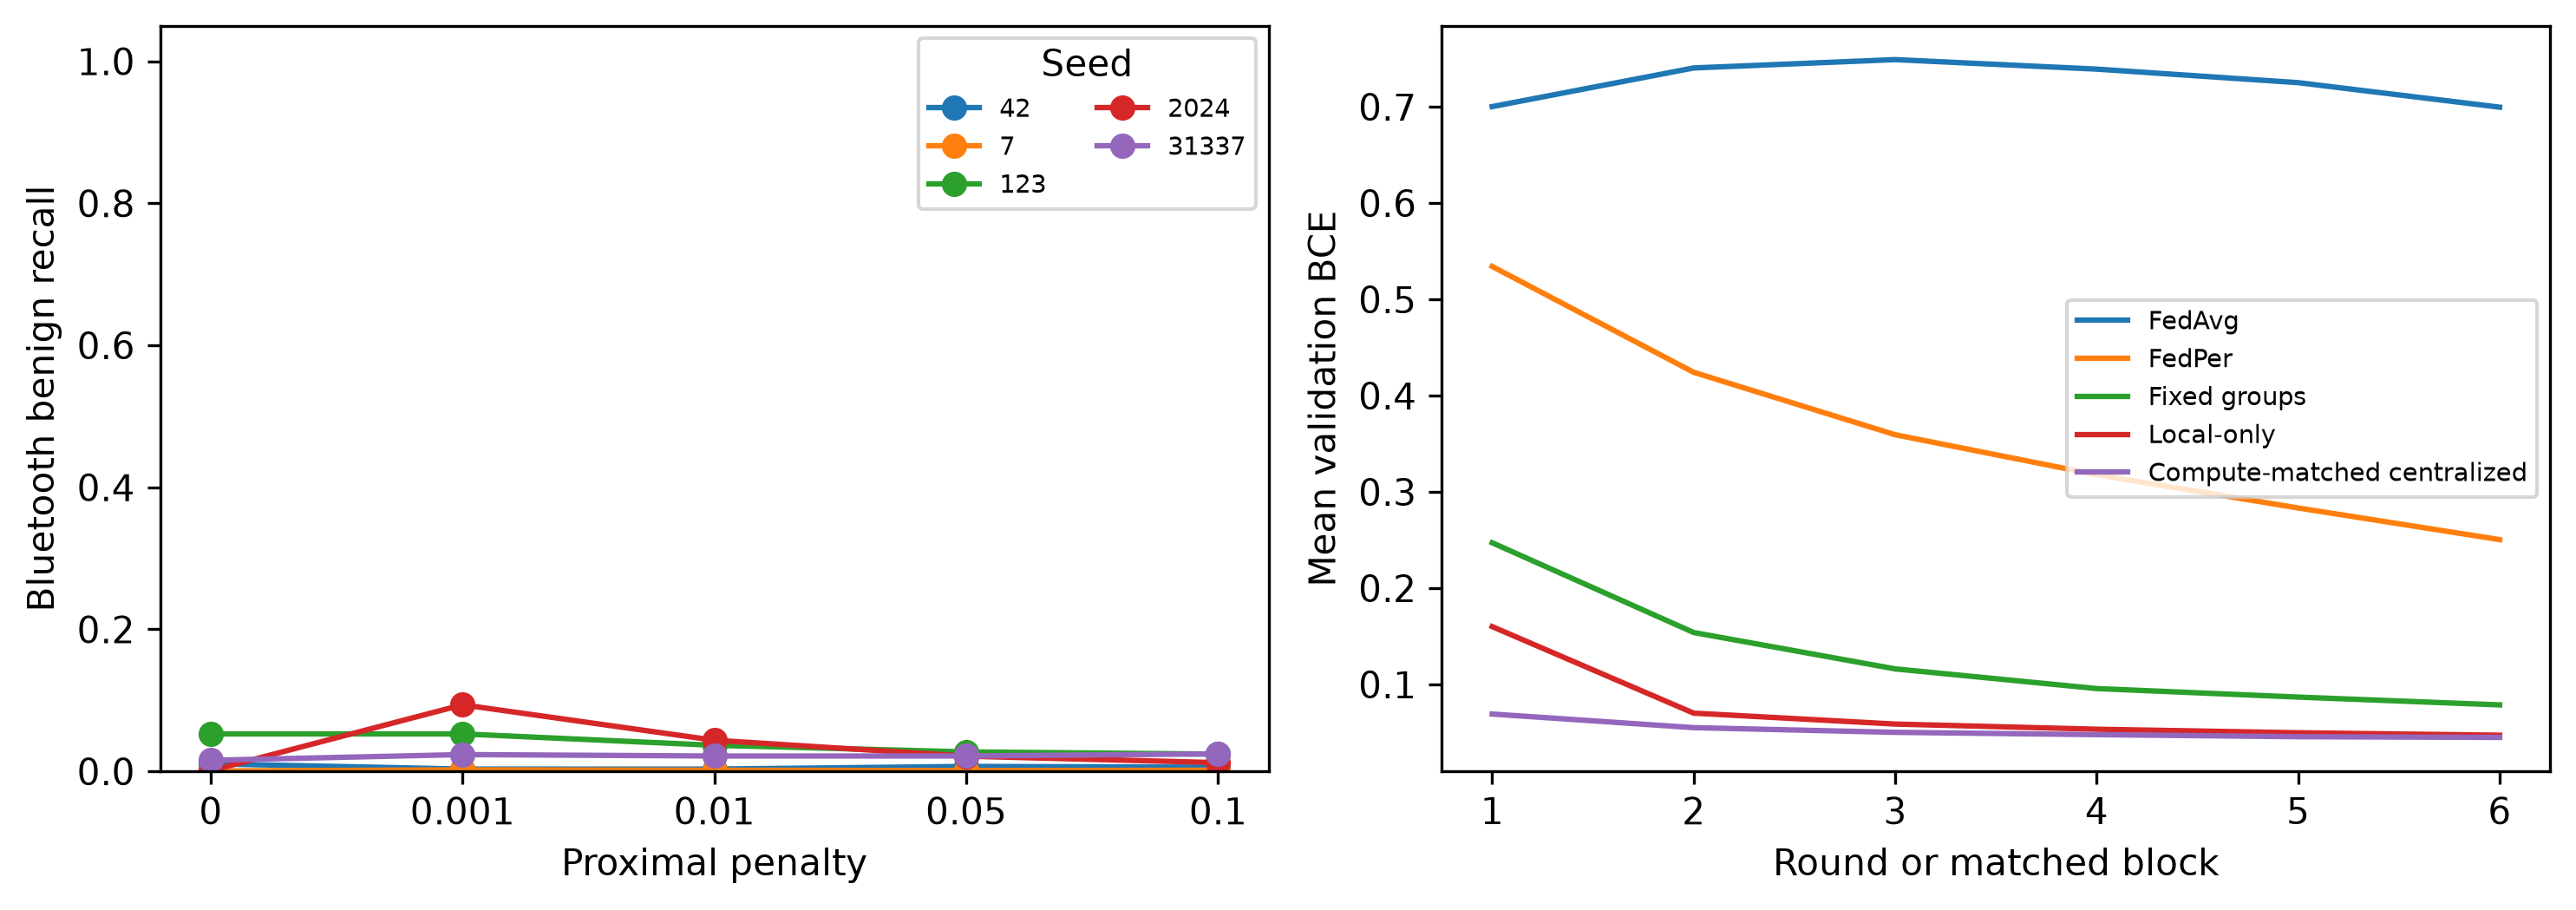
\includegraphics[width=0.93\textwidth]{revision_sweep_budget.png}
\caption{Left: test specificity for the proximal sweep. Right: validation binary cross-entropy averaged over clients and seeds.}\label{fig:revised_sweep_budget}
\end{figure*}
}

\newcommand{\RevisionDiagnostics}{%
\begin{table*}[t]\centering
\caption{Bluetooth diagnostics on 5 seeds, mean and sample standard deviation.}\label{tab:newprobe}
\resizebox{\textwidth}{!}{\begin{tabular}{lrrrrrr}\hline
Model & Specificity & Attack recall & Brier & ECE & ROC AUC & PR AUC\\\hline
fedavg & 0.0161 $\pm$ 0.0214 & 0.9982 $\pm$ 0.0022 & 0.3891 $\pm$ 0.0333 & 0.4602 $\pm$ 0.0338 & 0.8956 $\pm$ 0.0828 & 0.7576 $\pm$ 0.1452\\
threshold & 0.9619 $\pm$ 0.0190 & 0.3253 $\pm$ 0.4386 & 0.3891 $\pm$ 0.0333 & 0.4602 $\pm$ 0.0338 & 0.8956 $\pm$ 0.0828 & 0.7576 $\pm$ 0.1452\\
platt & 0.8370 $\pm$ 0.0952 & 0.9084 $\pm$ 0.0902 & 0.1007 $\pm$ 0.0470 & 0.1205 $\pm$ 0.0666 & 0.8956 $\pm$ 0.0828 & 0.7576 $\pm$ 0.1452\\
temperature & 0.0161 $\pm$ 0.0214 & 0.9982 $\pm$ 0.0022 & 0.2393 $\pm$ 0.0089 & 0.2933 $\pm$ 0.1007 & 0.8956 $\pm$ 0.0828 & 0.7576 $\pm$ 0.1452\\
fedper & 0.7180 $\pm$ 0.1016 & 0.9771 $\pm$ 0.0058 & 0.1297 $\pm$ 0.0287 & 0.2477 $\pm$ 0.0251 & 0.9739 $\pm$ 0.0091 & 0.9488 $\pm$ 0.0409\\
frozen trunk & 0.2577 $\pm$ 0.2387 & 0.9873 $\pm$ 0.0071 & 0.2332 $\pm$ 0.0322 & 0.3393 $\pm$ 0.0245 & 0.9624 $\pm$ 0.0272 & 0.9173 $\pm$ 0.0893\\
fine tune & 0.9903 $\pm$ 0.0045 & 0.9589 $\pm$ 0.0036 & 0.0220 $\pm$ 0.0027 & 0.0294 $\pm$ 0.0147 & 0.9810 $\pm$ 0.0031 & 0.9848 $\pm$ 0.0021\\
\hline\end{tabular}}
\end{table*}

\begin{figure*}[t]\centering
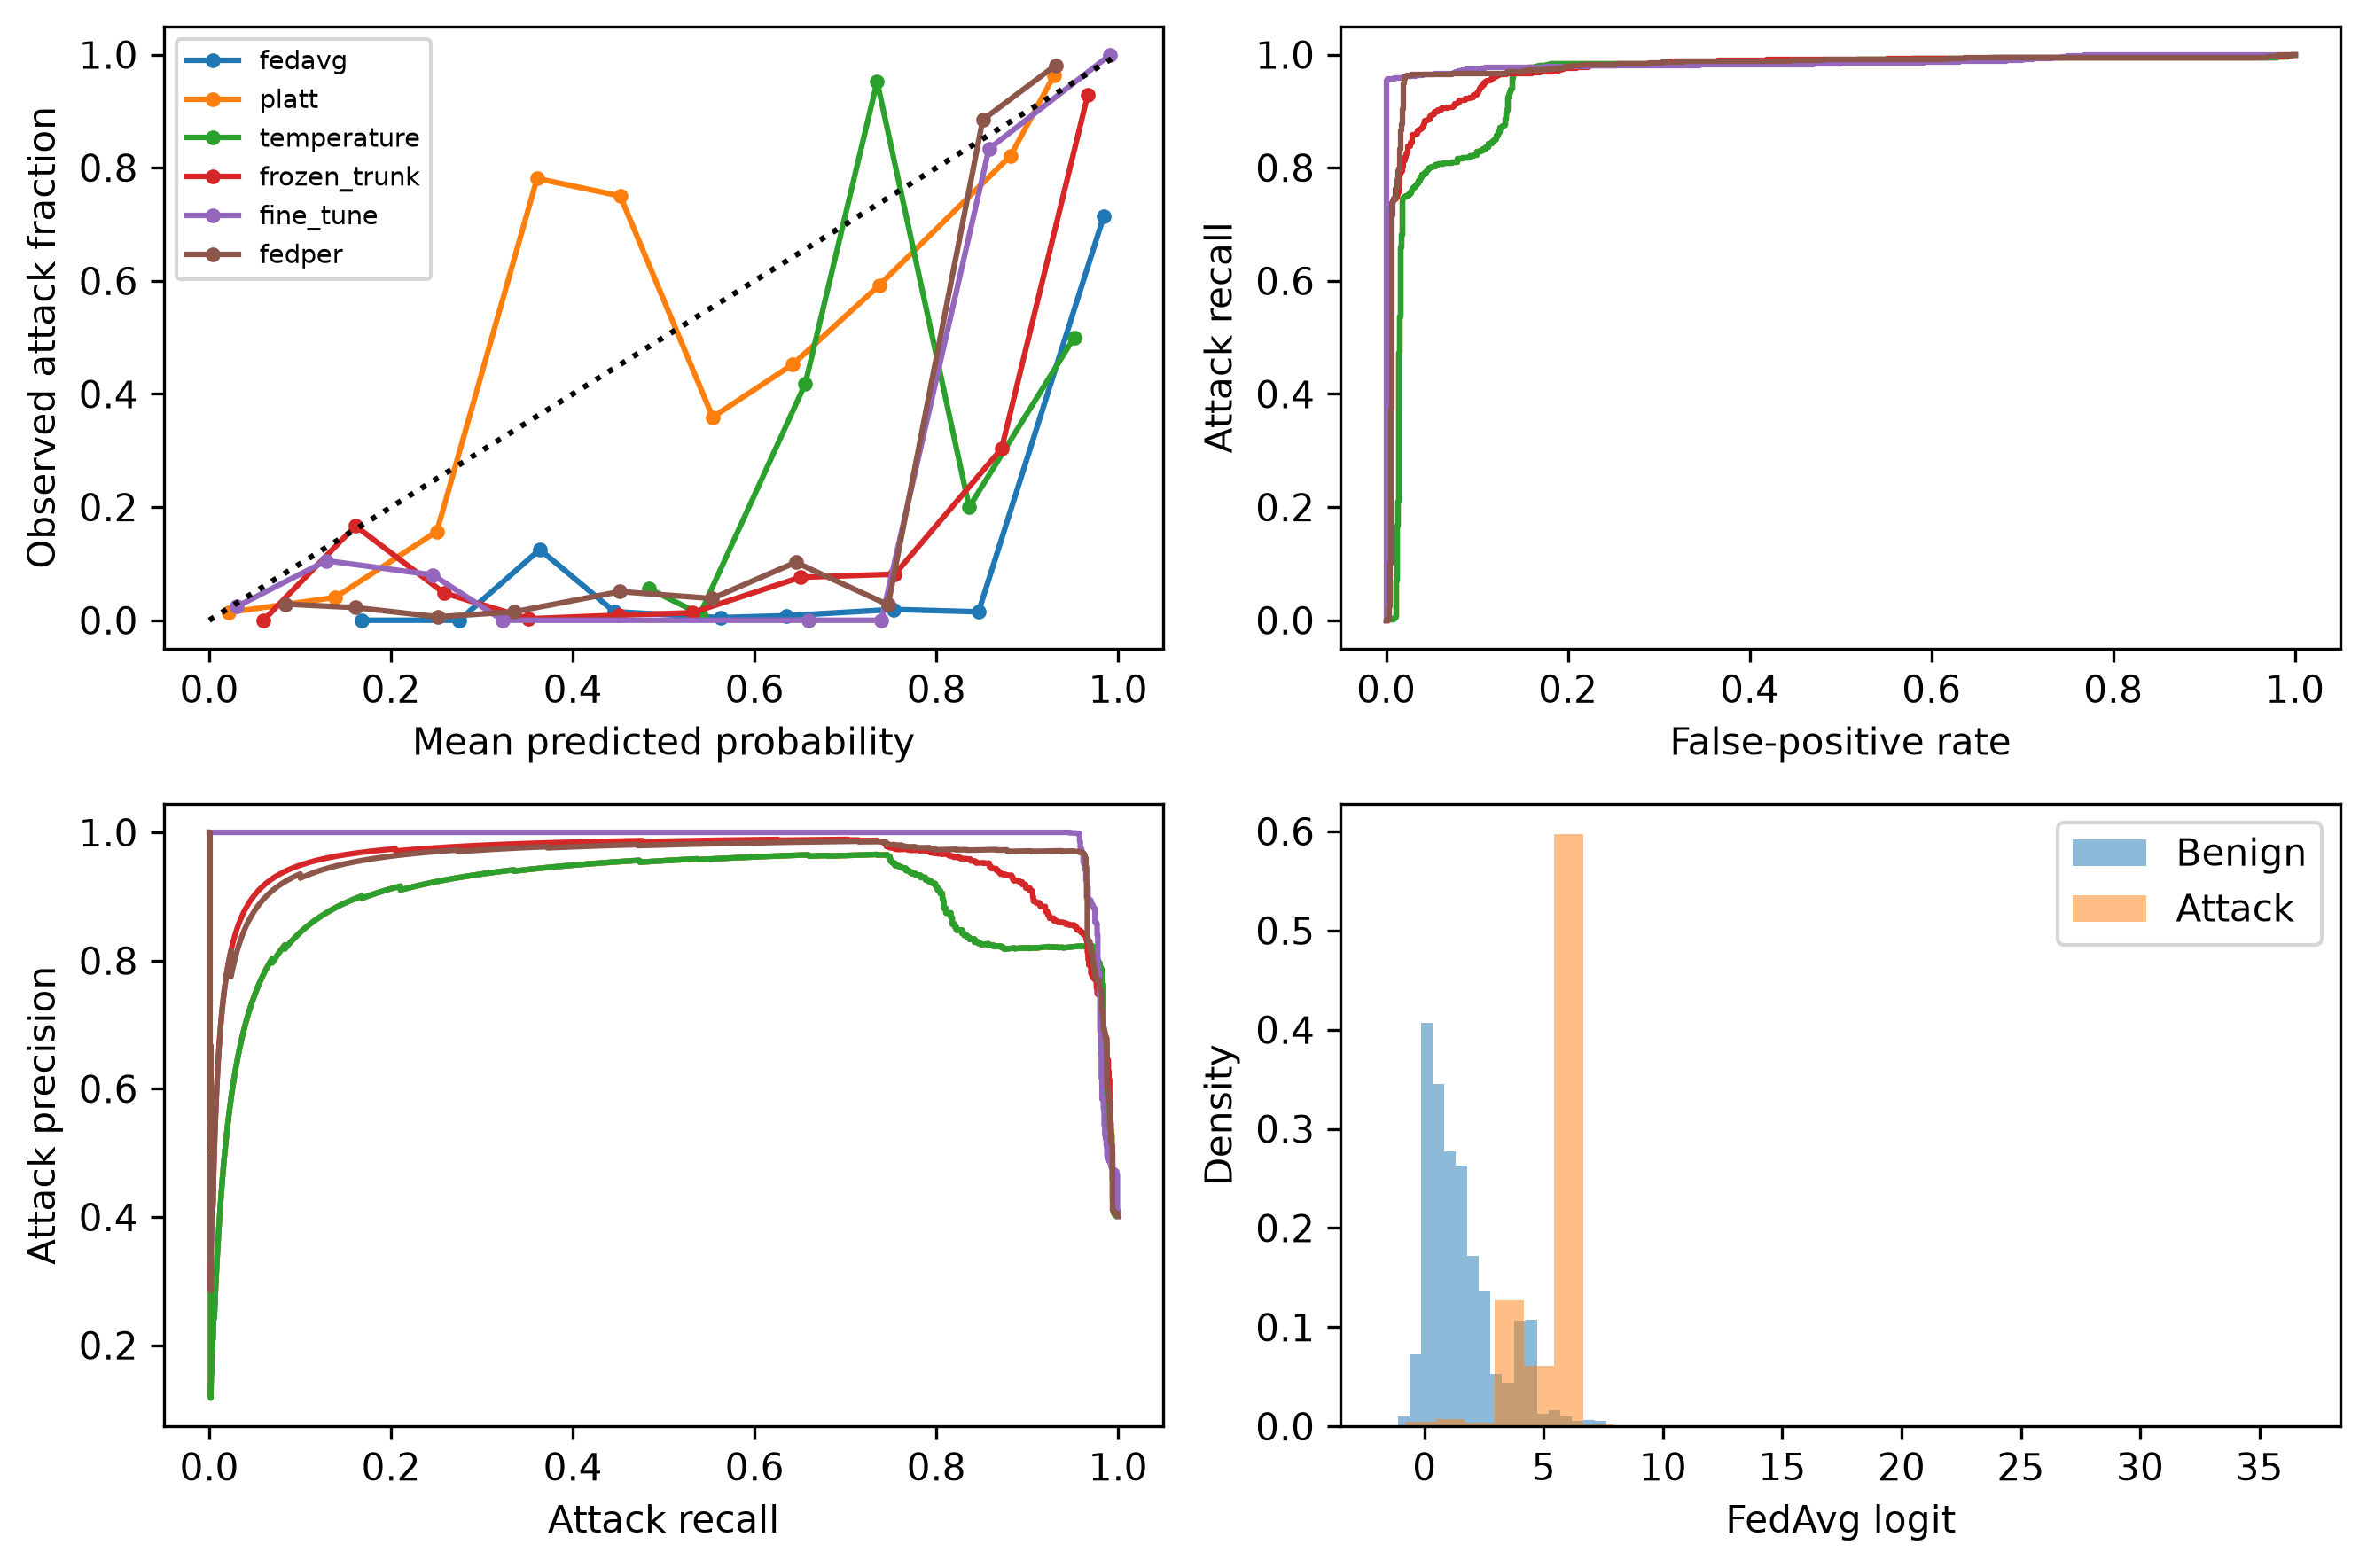
\includegraphics[width=0.93\textwidth]{revision_diagnostic.png}
\caption{Bluetooth score diagnostics for seed 123. Reliability, receiver operating characteristic, precision--recall, and the class-conditional FedAvg scores.}\label{fig:revised_diagnostic}
\end{figure*}
}

\newcommand{\RevisionShap}{%
\begin{table}[t]\centering
\caption{FedPer versus FedAvg within client on matched backgrounds and records.}\label{tab:newshapwithin}
\resizebox{\columnwidth}{!}{\begin{tabular}{lrrr}\hline
Client and class & Top-five Jaccard & Spearman & Cosine\\\hline
wifi benign & 0.6024 $\pm$ 0.2832 & 0.9606 $\pm$ 0.0414 & 0.9824 $\pm$ 0.0164\\
wifi attack & 0.6667 $\pm$ 0.0000 & 0.9521 $\pm$ 0.0400 & 0.9863 $\pm$ 0.0212\\
mqtt benign & 0.5905 $\pm$ 0.2511 & 0.9486 $\pm$ 0.0361 & 0.9810 $\pm$ 0.0205\\
mqtt attack & 0.7524 $\pm$ 0.2461 & 0.8976 $\pm$ 0.0331 & 0.9854 $\pm$ 0.0175\\
bluetooth benign & 0.5548 $\pm$ 0.2896 & 0.9835 $\pm$ 0.0080 & 0.8657 $\pm$ 0.0563\\
bluetooth attack & 0.4881 $\pm$ 0.1786 & 0.9843 $\pm$ 0.0093 & 0.9131 $\pm$ 0.0280\\
\hline\end{tabular}}
\end{table}

\begin{table}[t]\centering
\caption{Within-method comparisons across clients using client-specific backgrounds.}\label{tab:newshapacross}
\resizebox{\columnwidth}{!}{\begin{tabular}{lrrr}\hline
Pair and class & Top-five Jaccard & Spearman & Cosine\\\hline
wifi-mqtt benign & 0.2024 $\pm$ 0.1400 & 0.7968 $\pm$ 0.0224 & 0.9078 $\pm$ 0.0366\\
wifi-mqtt attack & 0.6857 $\pm$ 0.2037 & 0.7236 $\pm$ 0.0301 & 0.9671 $\pm$ 0.0093\\
wifi-bluetooth benign & 0.0444 $\pm$ 0.0609 & 0.4499 $\pm$ 0.0704 & 0.2013 $\pm$ 0.0329\\
wifi-bluetooth attack & 0.0222 $\pm$ 0.0497 & 0.2450 $\pm$ 0.0550 & 0.0947 $\pm$ 0.0096\\
mqtt-bluetooth benign & 0.0000 $\pm$ 0.0000 & 0.3224 $\pm$ 0.0638 & 0.1411 $\pm$ 0.0649\\
mqtt-bluetooth attack & 0.0444 $\pm$ 0.0609 & 0.1557 $\pm$ 0.0825 & 0.1126 $\pm$ 0.0572\\
\hline\end{tabular}}
\end{table}

\begin{figure*}[t]\centering
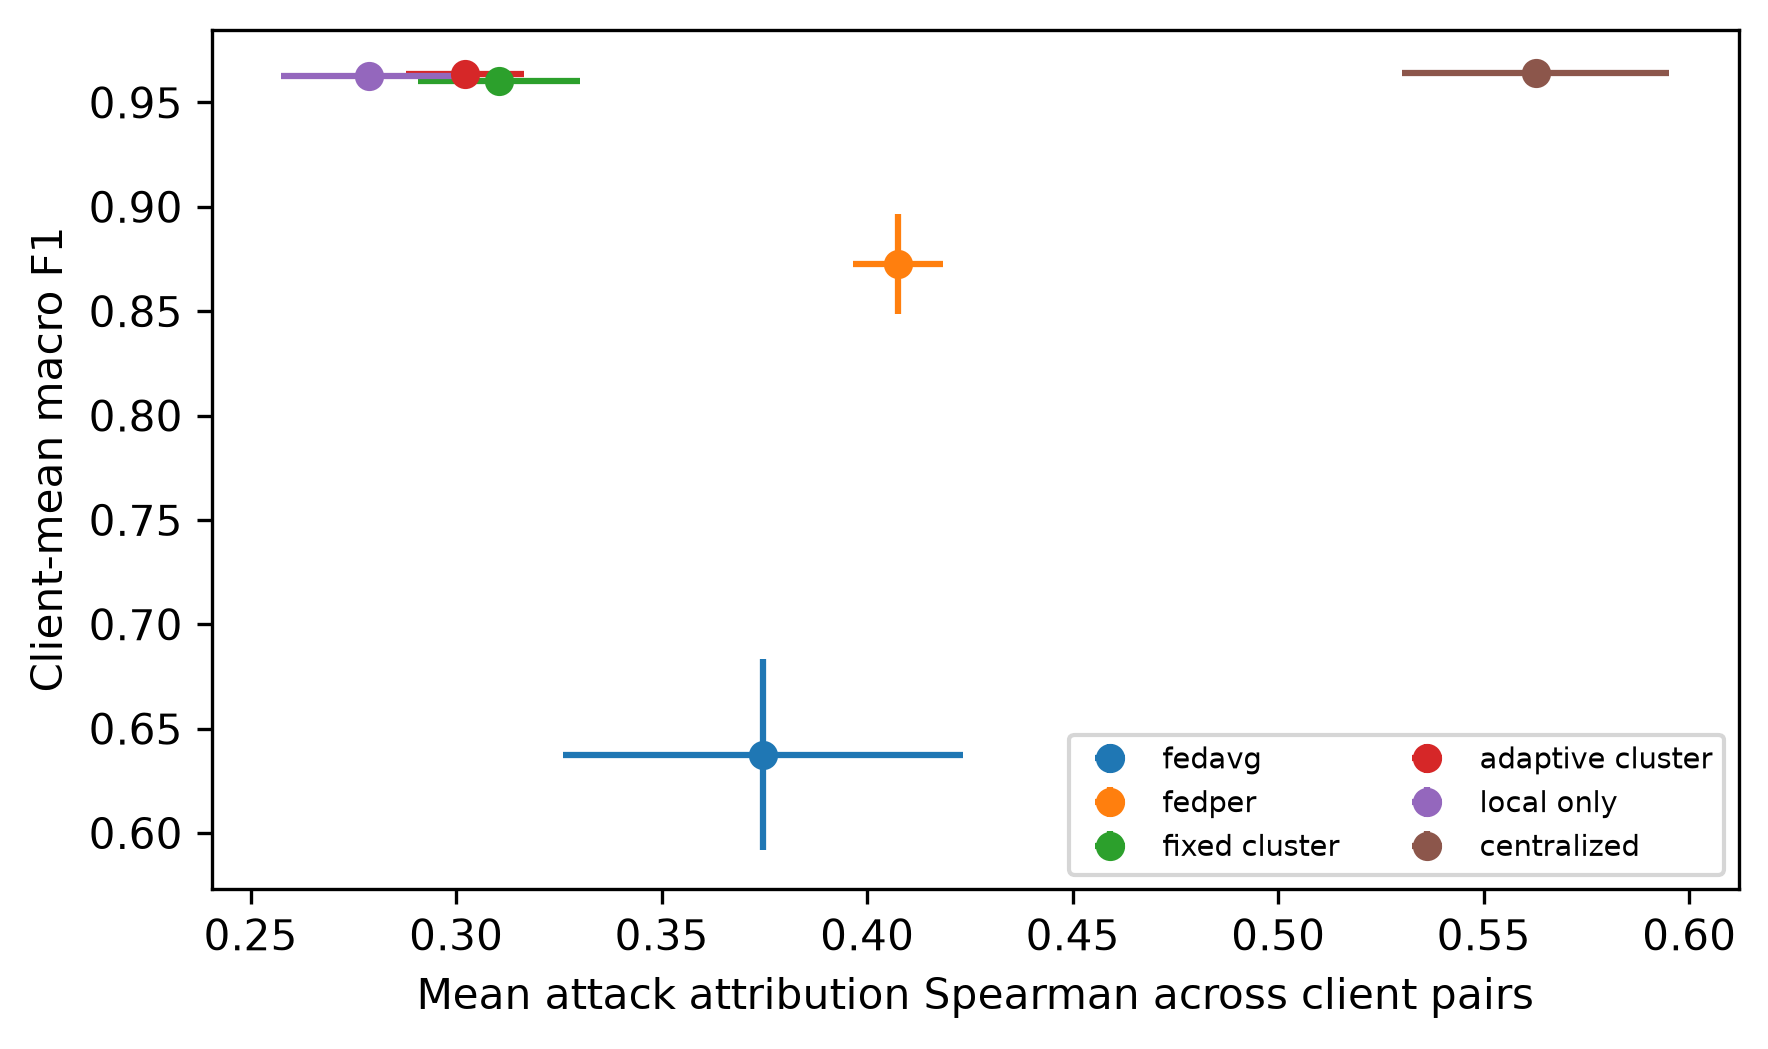
\includegraphics[width=0.93\textwidth]{revision_shap_tradeoff.png}
\caption{Each point averages over the available matched seeds. The horizontal statistic first averages the three within-method protocol pairs. Error bars are sample standard deviations across seeds.}\label{fig:revised_shap_tradeoff}
\end{figure*}
}

\newcommand{\RevisionSensitivity}{%
\begin{table*}[t]\centering
\caption{One-factor settings and the round-by-epoch interaction on the reduced budget.}\label{tab:newsensitivity}
\resizebox{\textwidth}{!}{\begin{tabular}{lrrrr}\hline
Setting & Seeds & Client mean macro F1 & BT specificity & BT Spearman\\\hline
anchor & 2 & 0.5752 $\pm$ 0.0021 & 0.0000 $\pm$ 0.0000 & 0.9927 $\pm$ 0.0009\\
batch 128 & 2 & 0.5989 $\pm$ 0.0023 & 0.0000 $\pm$ 0.0000 & 0.9933 $\pm$ 0.0015\\
batch 512 & 2 & 0.5458 $\pm$ 0.0076 & 0.0000 $\pm$ 0.0000 & 0.9914 $\pm$ 0.0018\\
dropout 0 & 2 & 0.6034 $\pm$ 0.0474 & 0.0003 $\pm$ 0.0004 & 0.9917 $\pm$ 0.0081\\
dropout 04 & 2 & 0.5733 $\pm$ 0.0054 & 0.0000 $\pm$ 0.0000 & 0.9922 $\pm$ 0.0034\\
epochs 1 & 2 & 0.5409 $\pm$ 0.0111 & 0.0000 $\pm$ 0.0000 & 0.9897 $\pm$ 0.0051\\
epochs 3 & 2 & 0.5975 $\pm$ 0.0046 & 0.0000 $\pm$ 0.0000 & 0.9939 $\pm$ 0.0013\\
head 1 & 2 & 0.7025 $\pm$ 0.0349 & 0.1159 $\pm$ 0.1046 & 0.9863 $\pm$ 0.0056\\
head 2 & 2 & 0.9606 $\pm$ 0.0003 & 0.9922 $\pm$ 0.0002 & 0.9760 $\pm$ 0.0083\\
interaction high & 2 & 0.5975 $\pm$ 0.0046 & 0.0000 $\pm$ 0.0000 & 0.9939 $\pm$ 0.0013\\
interaction long short & 2 & 0.6490 $\pm$ 0.0135 & 0.0056 $\pm$ 0.0071 & 1.0000 $\pm$ 0.0000\\
interaction low & 2 & 0.5409 $\pm$ 0.0111 & 0.0000 $\pm$ 0.0000 & 0.9897 $\pm$ 0.0051\\
interaction short long & 2 & 0.5975 $\pm$ 0.0046 & 0.0000 $\pm$ 0.0000 & 0.9939 $\pm$ 0.0013\\
lr high & 2 & 0.6317 $\pm$ 0.0307 & 0.0003 $\pm$ 0.0004 & 0.9948 $\pm$ 0.0010\\
lr low & 2 & 0.5433 $\pm$ 0.0050 & 0.0000 $\pm$ 0.0000 & 0.9914 $\pm$ 0.0018\\
rounds 2 & 2 & 0.5752 $\pm$ 0.0021 & 0.0000 $\pm$ 0.0000 & 0.9927 $\pm$ 0.0009\\
rounds 6 & 2 & 0.6126 $\pm$ 0.0550 & 0.0013 $\pm$ 0.0018 & 0.9933 $\pm$ 0.0017\\
width double & 2 & 0.6086 $\pm$ 0.0108 & 0.0019 $\pm$ 0.0026 & 0.9933 $\pm$ 0.0006\\
width half & 2 & 0.5402 $\pm$ 0.0065 & 0.0000 $\pm$ 0.0000 & 0.9809 $\pm$ 0.0043\\
\hline\end{tabular}}
\end{table*}

\begin{figure*}[t]\centering
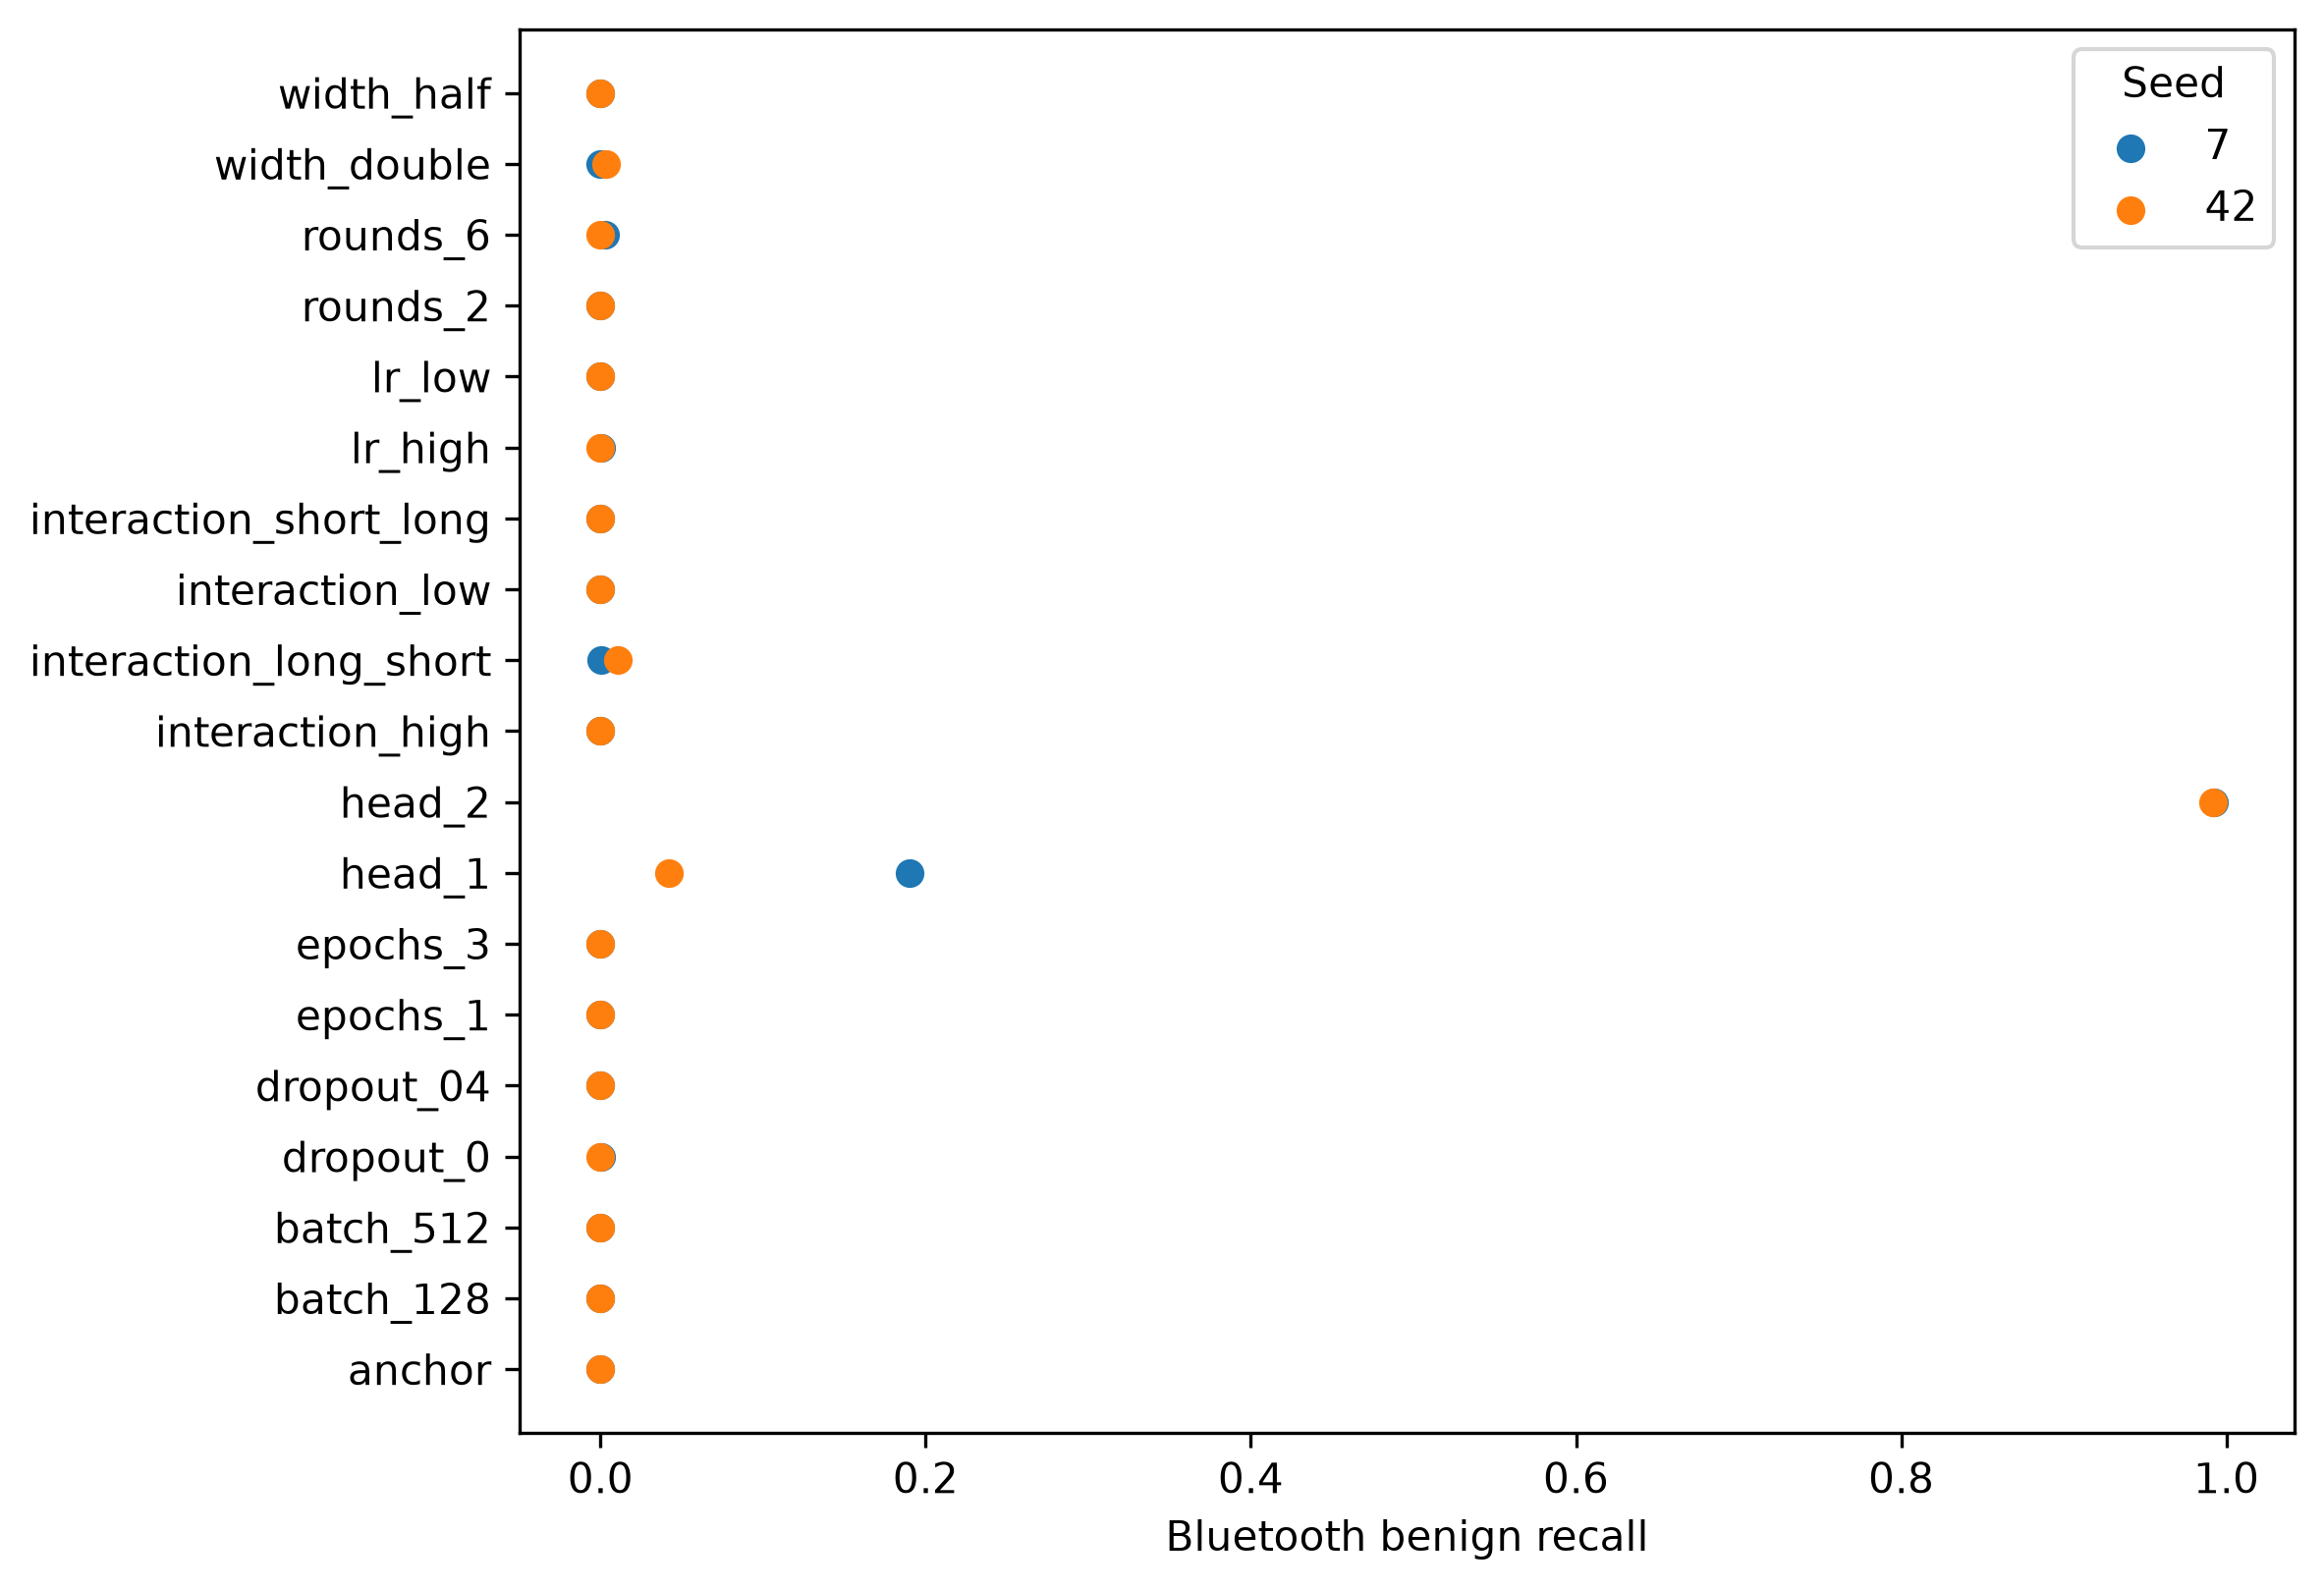
\includegraphics[width=0.93\textwidth]{revision_sensitivity.png}
\caption{Bluetooth benign recall across tested sensitivity configurations.}\label{fig:revised_sensitivity}
\end{figure*}
}

\newcommand{\RevisionTransfer}{%
\begin{table}[t]\centering
\caption{Foreign-feature transfer to the Bluetooth model. Attack metrics weight source labels equally.}\label{tab:newtransfer}
\resizebox{\columnwidth}{!}{\begin{tabular}{lrrr}\hline
Target model & Attack recall & Source-mean benign FPR & Detection margin\\\hline
FedAvg & 0.9915 & 1.0000 & -0.0085\\
FedPer & 0.9031 & 0.9715 & -0.0684\\
Fixed groups & 0.7763 & 0.9537 & -0.1767\\
Adaptive groups & 0.5764 & 0.9505 & -0.3734\\
Local-only & 0.1058 & 0.1643 & -0.0582\\
Centralized & 0.9455 & 0.9882 & -0.0428\\
\hline\end{tabular}}
\end{table}

\begin{table}[t]\centering
\caption{Binary recall on the omitted reconnaissance labels. Each retained test label has equal weight.}\label{tab:newholdout}
\small\begin{tabular}{lrr}\hline
Training method & Seeds & Reconnaissance recall\\\hline
Adaptive groups & 2 & 0.8931 $\pm$ 0.0143\\
Centralized & 2 & 0.9022 $\pm$ 0.0601\\
Compute-matched centralized & 2 & 0.9047 $\pm$ 0.0491\\
Class-balanced loss & 2 & 0.5847 $\pm$ 0.0365\\
Equal client weights & 2 & 0.5967 $\pm$ 0.0214\\
FedAvg & 2 & 0.6824 $\pm$ 0.0315\\
FedPer & 2 & 0.7906 $\pm$ 0.0449\\
FedProx 0 & 2 & 0.6824 $\pm$ 0.0315\\
FedProx 0.001 & 2 & 0.6384 $\pm$ 0.0202\\
FedProx 0.01 & 2 & 0.6362 $\pm$ 0.0222\\
FedProx 0.05 & 2 & 0.6265 $\pm$ 0.0237\\
FedProx 0.1 & 2 & 0.6252 $\pm$ 0.0209\\
Fixed groups & 2 & 0.9027 $\pm$ 0.0225\\
Local-only & 2 & 0.8723 $\pm$ 0.0115\\
\hline\end{tabular}
\end{table}
}

\newcommand{\RevisionScarcity}{%
\begin{figure*}[t]\centering
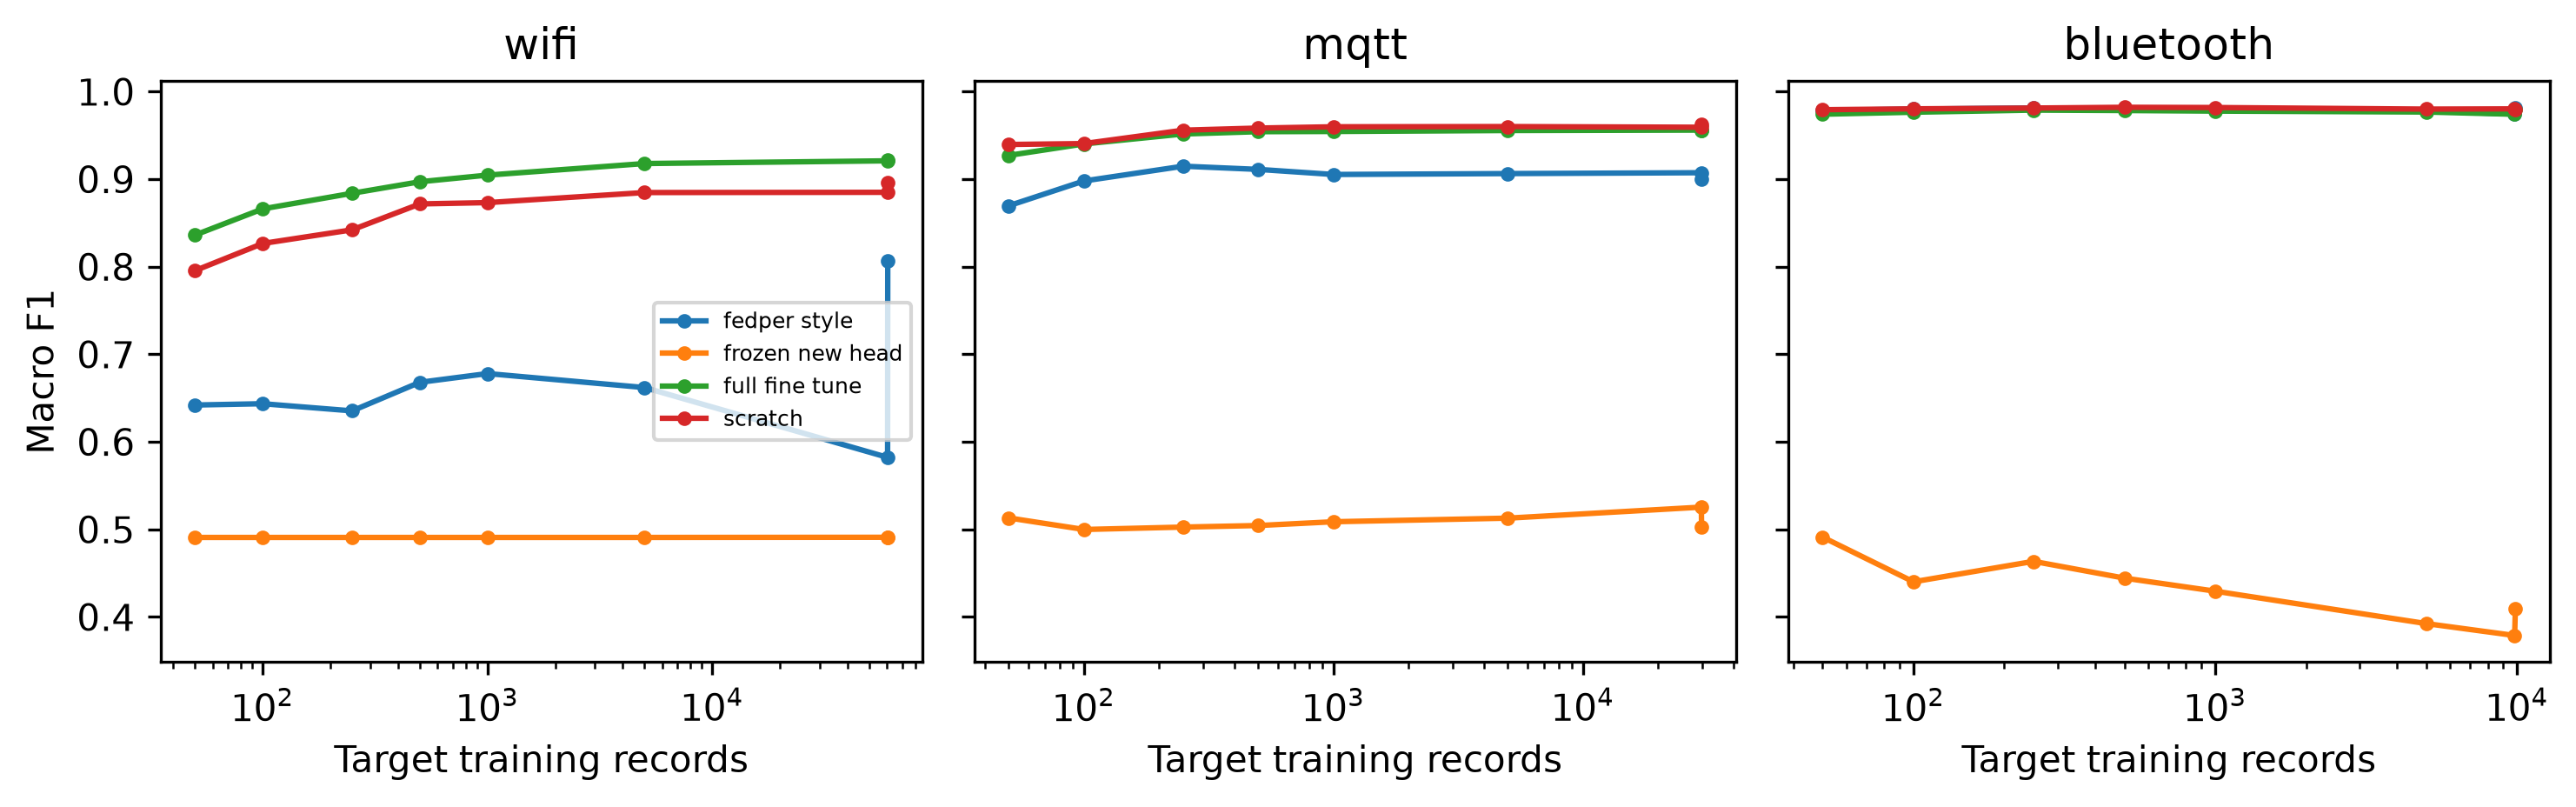
\includegraphics[width=0.93\textwidth]{revision_scarcity.png}
\caption{Target-excluded adaptation by budget and protocol. Full budgets can differ by seed.}\label{fig:revised_scarcity}
\end{figure*}
}
